\subsection{IP2D and IP3D}

\subsubsection{Lifetime signage}

\begin{figure}[htbp]
  \centering
 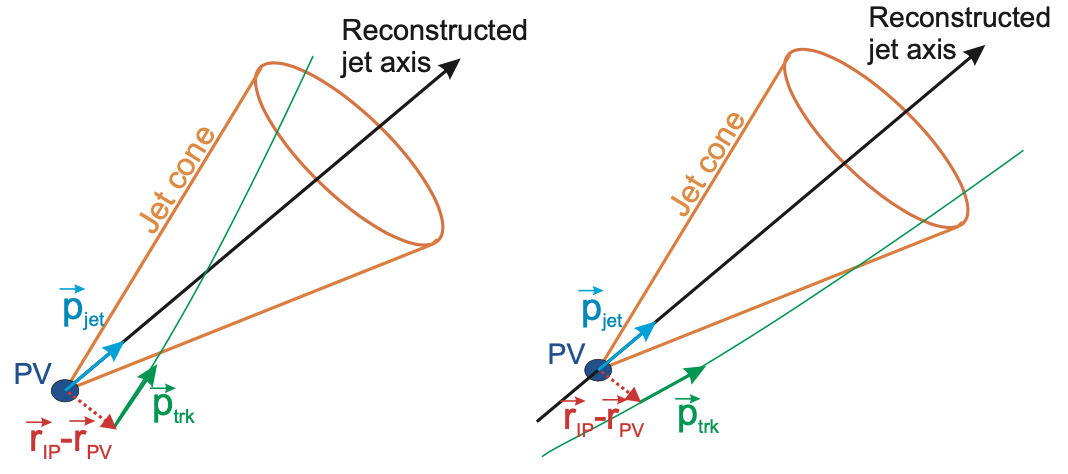
\includegraphics[width=0.5\textwidth]{figures/ftag/lifetime-signage}
 \caption{Lifetime signage graphic (from \cite{giacinto-thesis})}
 \label{fig:lifetime-signage}
\end{figure}


\textbf{3d sign}

$\Delta \vec{r}_{IP} = \vec{r}_{IP}  - \vec{r}_{PV} $

\begin{equation}
  \text{sign}_{3D} =   \text{sign} \left( \left[ \vec{p}_{trk} \times \vec{p}_{jet} \right] \cdot \left[   \vec{p}_{trk} \times \Delta \vec{r}_{IP} \right] \right)
  %\label{eq:}
\end{equation}

\textbf{2d sign}

\begin{equation}
  \text{sign}_{r \phi} =   \text{sign} \left( \sin \left( \phi_{jet} - \phi_{trk} \right) \cdot d_{0,trk} \right)
  %\label{eq:}
\end{equation}

\begin{equation}
  \text{sign}_{z} =   \text{sign} \left(  \left(  \eta_{jet} - \eta_{trk} \right) \cdot z_{0,trk}  \right)
  %\label{eq:}
\end{equation}



(Equations taken from Giacinto's thesis  \cite{giacinto-thesis}.)

\textbf{How are the IPs signed for the IP2D and IP3D algorithms}

\begin{itemize}
	\item \textbf{IP2D: }
	\begin{itemize}
	\item$d_0$ signed based on the projection of the vectors in the (x,y) plane
	\end{itemize}

	\item \textbf{IP3D:}
	\begin{itemize}
	\item $d_0$ signed with the 3D vectors
	\item $z_0$ signed based on the $(r, \phi)$ plane
\end{itemize}
\end{itemize}

\subsubsection{Mathematical motivation}


\begin{figure}[htbp]
  \centering
 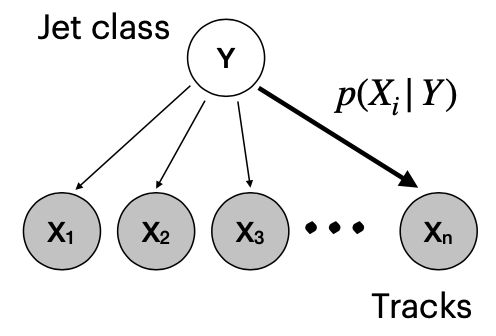
\includegraphics[width=0.5\textwidth]{figures/ftag/Naive-Bayes-illustration}
 \caption{Probabilistic graphical model illustration for a Naive Bayes algorithm.  }
  \label{fig:Naive-Bayes-illustration}
\end{figure}

%%%%%%%%%%%%%%%%%%%%%%%%%%%%
% Plot showing the non-independence of the tracking inputs
%%%%%%%%%%%%%%%%%%%%%%%%%%%%

%\def\figpath{figures/ftag/ATL-PHYS-PUB-2017-003/}
\begin{figure}[htbp]
  \centering
  \subfloat[]{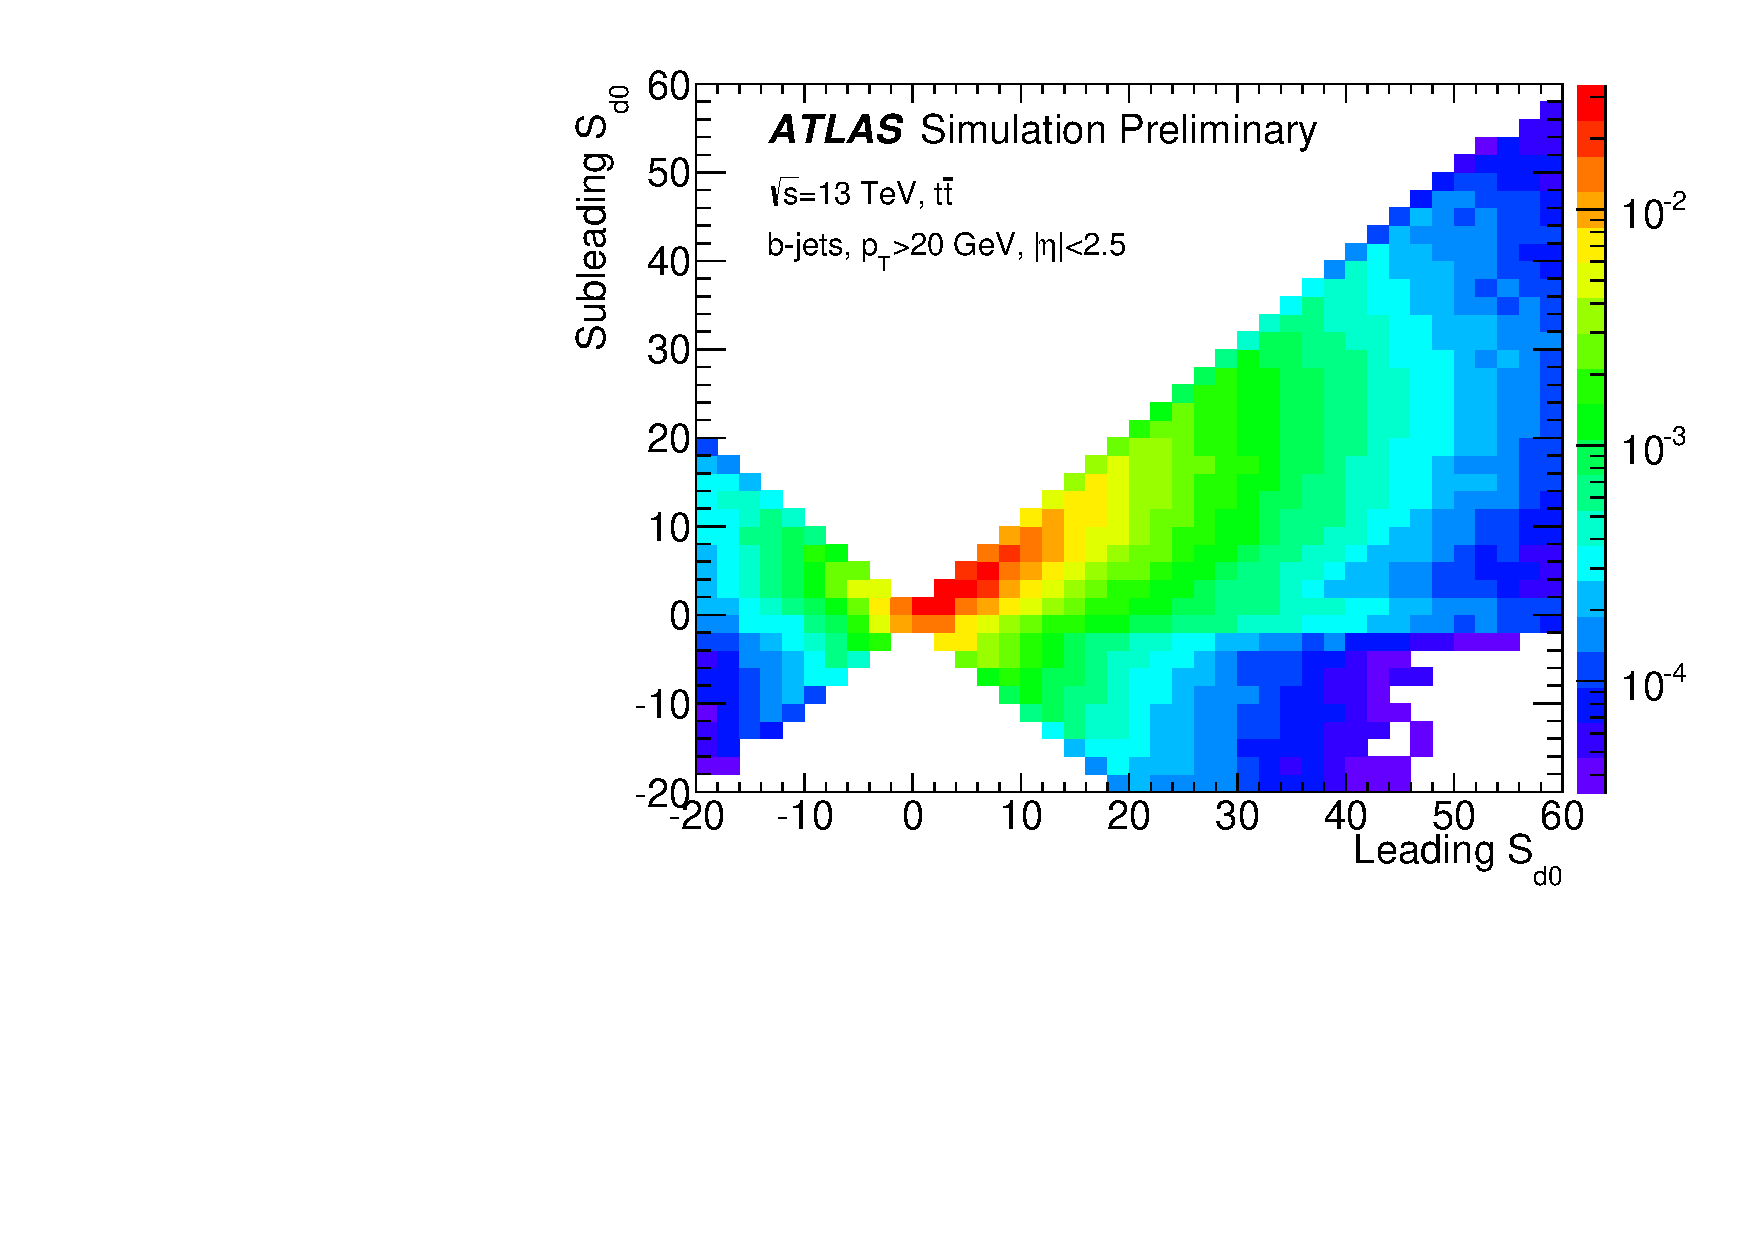
\includegraphics[width=0.5\textwidth]{figures/ftag/ATL-PHYS-PUB-2017-003/fig_01a}}
  \subfloat[]{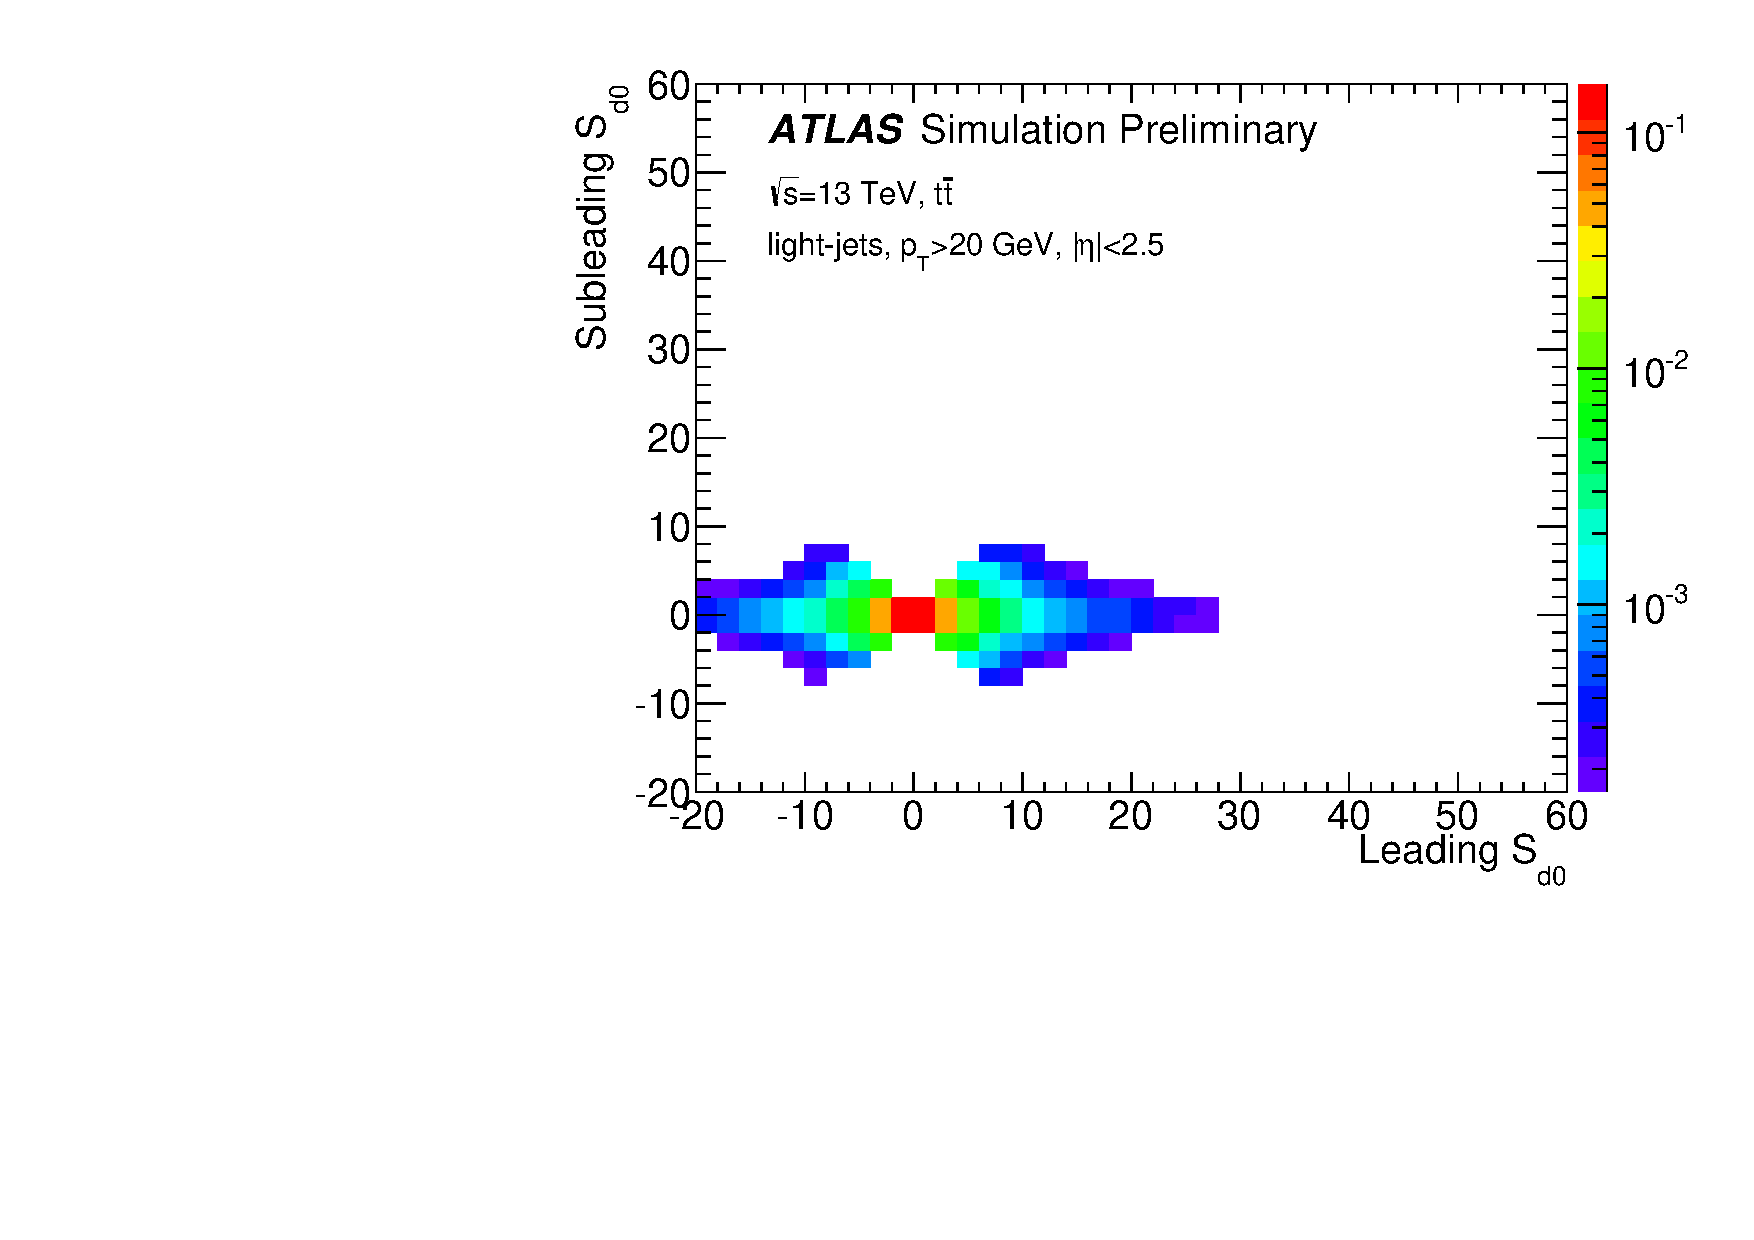
\includegraphics[width=0.5\textwidth]{figures/ftag/ATL-PHYS-PUB-2017-003/fig_01b}}
  \caption{ \cite{ATL-PHYS-PUB-2017-003}}
  \label{fig:rnnip-note-trk-ind}
\end{figure}


\subsubsection{Algorithm description}

% I don't think I need to describe the benefit of IP based algorithms
%\textbf{Should I mention that the lifetime signage is different between IP2D and IP3D? No - beyond the scope!}


The IP3D algorithm \cite{FTAG-2018-01} assigns probabilities to tracks based on two-dimensional likelihood templates, with the tracks' $z_0\sin\theta$ and $d_0$ lifetime signed significances, built from simulated jets.
These templates are obtained in 14 exclusive categories defined by the hit patterns of the tracks, and separately for tracks in $b$-jets, $c$-jets and light-flavour jets. 
The inclusive distribution of $z_0\sin\theta$ and $d_0$ lifetime signed significances for the different jet flavours are shown in Figure \ref{fig:flippedInputs}.
% The IP3D algorithm builds histograms for estimating the likelihood distribution of the IP significance for the tracks in $b$-jets and $l$-jets in 14 exclusive categories defined by the hit patterns of the tracks \cite{FTAG-2018-01}. 
By assuming that the track probabilities inside a jet are independent, jet-level likelihoods can be constructed by multiplying the individual probabilities.
The IP3D $b$-tagging discriminants are therefore defined as:
\begin{equation}
D_{\text{IP3D,l}} = \log \prod_{i \in \text{tracks}} \frac{p_b^i}{p_l^{i}} \qquad D_{\text{IP3D,c}} = \log \prod_{i \in \text{tracks}} \frac{p_b^i}{p_c^{i}}.
\end{equation}
% multiplication over the track likelihoods produces a jet level probability, and the ratio of jet probabilities from the $l$ and $b$ hypotheses defines the $b$-tagging discriminant: $\log \prod_{i \in tracks} p_b^{(i)} / p_l^{(i)}$.
RNN based IP algorithms aim to overcome this overly simplistic assumption of independence, and offer the possibility to employ more features than only the IP significance in the discriminant~\cite{ATL-PHYS-PUB-2017-003}. 

%%%%%%%%%%%%%%%%%%%%%%%%%%%%
% Plot from the DIPS note
%%%%%%%%%%%%%%%%%%%%%%%%%%%%
\def\figpath{figures/ftag/dips-note/}
\begin{figure}[htbp]
  \centering
  \subfloat[]{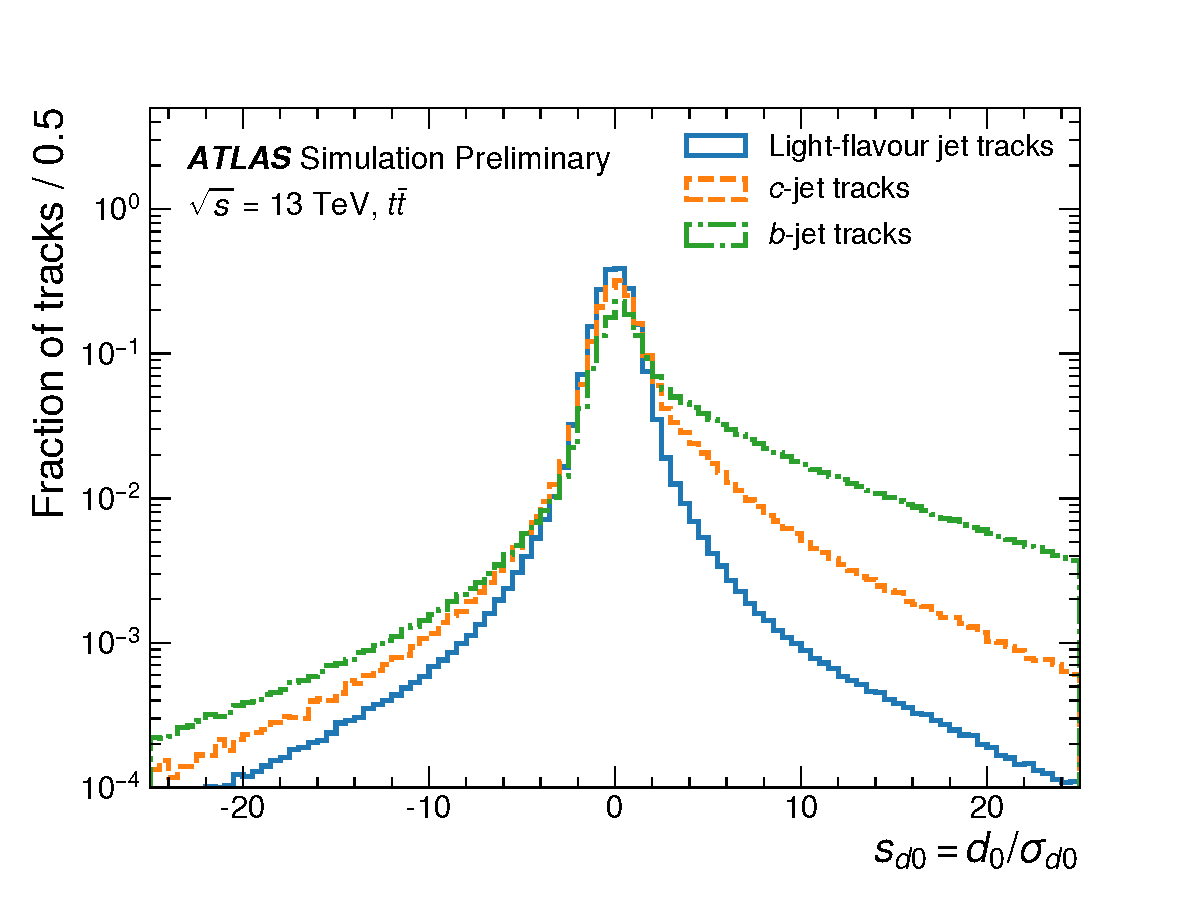
\includegraphics[width=0.5\textwidth]{\figpath/sd0}}
  \subfloat[]{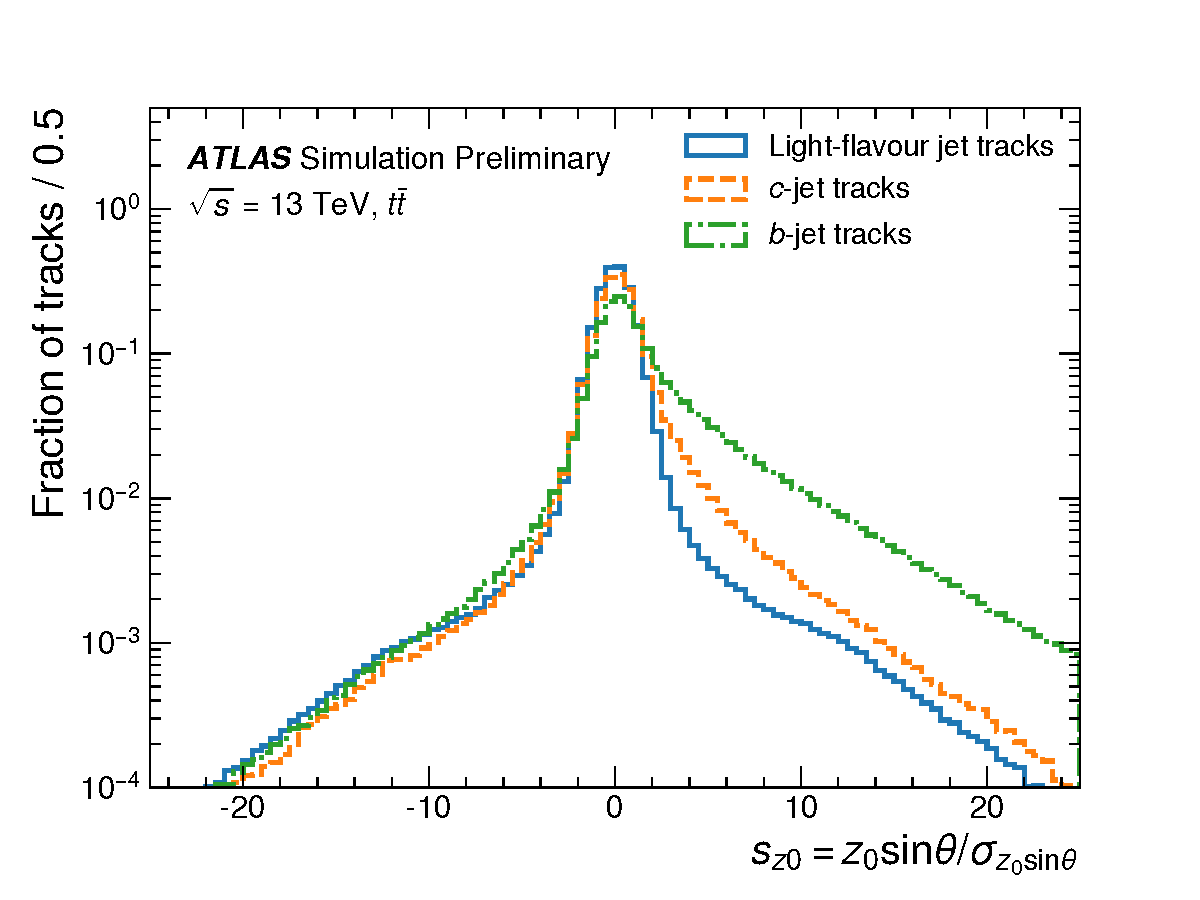
\includegraphics[width=0.5\textwidth]{\figpath/sz0}}
  \caption{Lifetime signed transverse (a) and longitudinal (b) significances for $b$-jets, $c$-jets and light-flavor jets.}
  \label{fig:flippedInputs}
\end{figure}

%%%%%%%%%%%%%%%%%%%%%%%%%%%%%%%%
% Table of the IPXD categories
%%%%%%%%%%%%%%%%%%%%%%%%%%%%%%%%

\begin{table}[h!]
  \begin{center}
    \begin{adjustbox}{width=\columnwidth,center}
    \begin{tabular}{ l | l | c c c  } % <-- Alignments: 1st 2 cols left, last three 3rd right, with vertical lines in between
      {} & {} &  \multicolumn{3}{ c }{ Fractional contribution [\%] } \\
      \textbf{\#} & \textbf{Category}  & \Pqb-jets & \Pqc-jets & light-jets  \\
      \midrule 
      0 & No hits in first two layers; expected hit in IBL and b-layer & 1.9 & 2.0 & 1.9   \\
      1 & No hits in first two layers; expected hit in IBL and no expected hit in b-layer & 0.1 & 0.1 & 0.1 \\
      2 & No hits in first two layers; no expected hit in IBL and expected hit in b-layer & 0.04 & 0.04 & 0.04 \\
      3 & No hits in first two layers; no expected hit in IBL and b-layer & 0.03 & 0.03 & 0.03 \\
      4 & No hit in IBL; expected hit in IBL & 2.4 & 2.3 & 2.1 \\
      5 & No hit in IBL; no expected hit in IBL & 1.0 & 1.0 & 0.9  \\
      6 & No hit in b-layer; expected hit in b-layer & 0.5 & 0.5 & 0.5 \\
      7 & No hit in b-layer; no expected hit in b-layer & 2.4 & 2.4 & 2.2  \\
      8 & \emph{Shared} hit in both IBL and b-layer & 0.01 & 0.01 & 0.03  \\
      9 & At least one \emph{shared} pixel hits & 2.0 & 1.7 & 1.5  \\
      10 & Two or more \emph{shared} SCT hits & 3.2 & 3.0 & 2.7  \\
      11 & \emph{Split} hits in both IBL and b-layer & 1.0 & 0.87 & 0.6  \\ 
      12 & \emph{Split} pixel hit & 1.8 & 1.4 & 0.9 \\
      13 & Good quality & 83.6 & 84.8 & 86.4 
    \end{tabular}
    \end{adjustbox}
    \caption{Categories for defining the IP2D and IP3D templates \cite{ATL-PHYS-PUB-2017-013}.}
    \label{table:IPXD-categories}
  \end{center}
\end{table}
